\documentclass[handout]{beamer}

\usetheme[progressbar=frametitle]{metropolis}
\usepackage{appendixnumberbeamer}
\usepackage{booktabs}
\usepackage{amsmath}
\usepackage{amssymb}
\usepackage{tcolorbox}
\usepackage{tikz}
\usetikzlibrary{bayesnet}
\definecolor{metropolisblue}{RGB}{39, 59, 94}



% Begin document
\begin{document}


% Title page
\title{Maximum Likelihood Estimation}
\author{Nipun Batra}
\date{\today}
\institute{IIT Gandhinagar}
\maketitle
\setbeamercovered{invisible}
\begin{frame}
    \frametitle{Agenda}
    \tableofcontents[hidesubsections]
    \end{frame}
    
\begin{section}{Revision - Prior, Posterior, MLE, MAP}
\end{section}
\begin{section}{Distributions, IID}
    \begin{frame}
        Notebook (distribution.ipynb)
    \end{frame}

    \begin{frame}{IID}
        \href{https://en.wikipedia.org/wiki/Independent_and_identically_distributed_random_variables}{Wiki Link}
    \end{frame}
        


    
    \begin{frame}{Graphical model}
        Assume model parameters are $\theta$ and data is $D  $. We can write the joint probability distribution as: \\
        \vspace{10pt}
        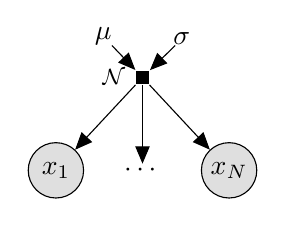
\begin{tikzpicture}
            \node[obs] (x1) {$x_1$};
            \node[const, right=0.5cm of x1]                               (dots) {$\cdots$};
            \node[obs, right=0.5cm of dots]                               (xn) {$x_N$};
            
            \factor[above=1 of dots] {y-f} {left:${\mathcal{N}}$} {} {} ; %
            \node[const, above=1.5 of dots, xshift=0.5cm] (sigma) {$\mathbf{\sigma}$};
            \node[const, above=1.5 of dots, xshift=-0.5cm] (mu) {$\mathbf{\mu}$};
            \edge {y-f} {dots} ;
            \edge {y-f} {xn} ; %
            \edge {y-f} {x1} ;
            \edge {mu, sigma} {y-f} ; %           
            
        \end{tikzpicture}
        
    \end{frame}

    \begin{frame}{Graphical model}
        Assume model parameters are $\theta$ and data is $D  $. We can write the joint probability distribution as:

        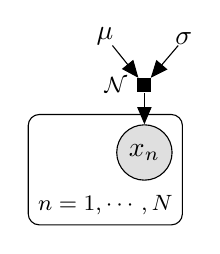
\begin{tikzpicture}
                
                
            \node[obs]                               (xn) {$x_n$};
            \factor[above=of xn] {y-f} {left:${\mathcal{N}}$} {} {} ; %
            \node[const, above=1 of xn, xshift=0.5cm] (sigma) {$\mathbf{\sigma}$};
            \node[const, above=1 of xn, xshift=-0.5cm] (mu) {$\mathbf{\mu}$};
            \plate{}{(xn)}{$n = 1, \cdots, N$};
            
            
            
            \edge {y-f} {xn} ; %
            \edge {mu, sigma} {y-f} ; %
            
            
        \end{tikzpicture}
        
    \end{frame}

    \begin{frame}{Factorisation of Likelihood}
        \begin{align*}
            P(D|\theta) & = P(x_1, x_2, \ldots, x_n | \theta) \\
            & = P(x_1|\theta) \cdot P(x_2|\theta) \cdot \ldots \cdot P(x_n|\theta)
        \end{align*}
        
    \end{frame}

\end{section}

\section{MLE}
\begin{frame}{Pop Quiz}
    We have three courses: C1, C2, C3. Assume no student takes more than one course.
    The scores of students in these courses are normally distributed with the following parameters:
    \begin{itemize}
        \item C1: $\mu_1 = 80, \sigma_1 = 10$
        \item C2: $\mu_2 = 70, \sigma_2 = 10$
        \item C3: $\mu_3 = 90, \sigma_3 = 5$
    \end{itemize}


    
\end{frame}

\begin{frame}{Pop Quiz}
    We have three courses: C1, C2, C3. Assume no student takes more than one course.
    The scores of students in these courses are normally distributed with the following parameters:
    \begin{itemize}
        \item C1: $\mu_1 = 80, \sigma_1 = 10$
        \item C2: $\mu_2 = 70, \sigma_2 = 10$
        \item C3: $\mu_3 = 90, \sigma_3 = 5$
    \end{itemize}

   
    I randomly pick up a student and ask them their marks. They say 82. Which course do you think they are from?
    To keep things simple, for now assume that all three courses have equal number of students.
    
    
    
\end{frame}

\begin{frame}{Pop Quiz}
    We have three courses: C1, C2, C3. Assume no student takes more than one course.
    The scores of students in these courses are normally distributed with the following parameters:
    \begin{itemize}
        \item C1: $\mu_1 = 80, \sigma_1 = 10$
        \item C2: $\mu_2 = 70, \sigma_2 = 10$
        \item C3: $\mu_3 = 90, \sigma_3 = 5$
    \end{itemize}

   
    I randomly pick up a student and ask them their marks. They say 82. Which course do you think they are from?
    
    
    
    Most likely C1. But why?
    
\end{frame}

\begin{frame}{Pop Quiz}
    Let us plot the probability density functions of the three courses. 
    \begin{figure}
        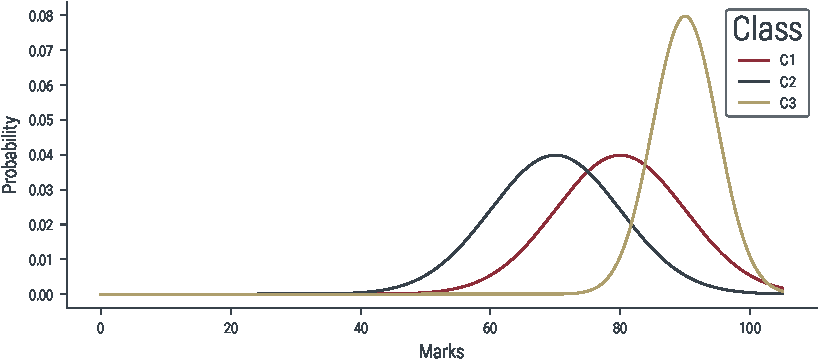
\includegraphics[width=\textwidth]{../figures/mle/mle-example.pdf}
    \end{figure}
    
\end{frame}

\begin{frame}{Pop Quiz}
    Let us plot the probability density functions of the three courses. 
    \begin{figure}
        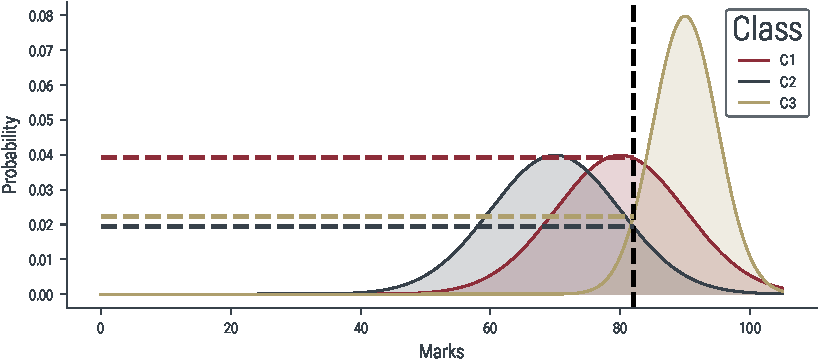
\includegraphics[width=\textwidth]{../figures/mle/mle-example-2.pdf}
    \end{figure}
    
\end{frame}

\begin{frame}
  Notebook (bayes-librarian.ipynb)
\end{frame}

\begin{frame}{Pop Quiz 2}
    Let us say we observed a value of 20. We know it came from a normal distribution with $\sigma=1$. What is the most likely value of $\mu$?
    


\end{frame}

\begin{frame}{Pop Quiz 2}
    Let us say we observed a value of 20. We know it came from a normal distribution with $\sigma=1$. What is the most likely value of $\mu$?
    
    20. But why?


\end{frame}

\begin{frame}{Pop Quiz 2}
    Let us say we observed a value of 20. We know it came from a normal distribution with $\sigma=1$. What is the most likely value of $\mu$?
    
    20. But why?

    Let us evaluate probability density function at 20 for different values of $\mu$ for $\sigma=1$, i.e., $f(x=20|\mu, \sigma=1)$.


\end{frame}

\begin{frame}{Pop Quiz 2}
    Let us say we observed a value of 20. We know it came from a normal distribution with $\sigma=1$. What is the most likely value of $\mu$?
    
    20. But why?

    Let us evaluate probability density function at 20 for different values of $\mu$ for $\sigma=1$, i.e., $f(x=20|\mu, \sigma=1)$.

    Importantly, this is a function of $\mu$ and not $x$ (which is fixed at 20).

\end{frame}

\begin{frame}
   Notebook (mle-univariate.ipynb)
\end{frame}

\begin{frame}{Pop Quiz 3}


Let us now go back to our original problem. We have three courses: C1, C2, C3. Assume no student takes more than one course.

We ask two students their marks. The first student says 82 and the second student says 72. Which course do you think they are from? Assumption: Both are from the same course.

Let us create a table of probabilities for each course:




    
\end{frame}

% Section 1
\section{MLE for Univariate Normal Distribution}

\begin{frame}{Univariate Normal Distribution}
The probability density function of a univariate normal distribution is given by:

\begin{equation}
f(x|\mu, \sigma^2) = \frac{1}{\sqrt{2\pi\sigma^2}}\exp\left(-\frac{(x-\mu)^2}{2\sigma^2}\right)
\end{equation}

Let us assume we have a dataset $D = \{x_1, x_2, \ldots, x_n\}$, where each $x_i$ is an independent sample from the above distribution. 
We want to estimate the parameters $\theta = \{\mu, \sigma\}$ from the data.

Our likelihood function is given by:
\begin{equation}
P(D|\theta) = \mathcal{L}(\mu, \sigma^2) = \prod_{i=1}^n f(x_i|\mu, \sigma^2)
\end{equation}


\end{frame}

\begin{frame}{Log Likelihood Function}
    Log-likelihood function:
    \begin{equation}
        \log \mathcal{L}(\mu, \sigma^2) = \sum_{i=1}^n \log f(x_i|\mu, \sigma^2)
    \end{equation}

    Simplifying the above equation, we get:
    \begin{align*}
        \log \mathcal{L}(\mu, \sigma^2) &= \sum_{i=1}^n \log f(x_i|\mu, \sigma^2) \\
        &= \sum_{i=1}^n \log \left( \frac{1}{\sqrt{2\pi\sigma^2}} \exp \left( -\frac{(x_i-\mu)^2}{2\sigma^2} \right) \right) \\
        &= \sum_{i=1}^n \left( \log \left( \frac{1}{\sqrt{2\pi\sigma^2}} \right) + \log \left( \exp \left( -\frac{(x_i-\mu)^2}{2\sigma^2} \right) \right) \right) \\
        \end{align*}
\end{frame}

\begin{frame}
   
    \begin{align*}
        \log \mathcal{L}(\mu, \sigma^2) &= \sum_{i=1}^n \left( \log \left( \frac{1}{\sqrt{2\pi\sigma^2}} \right) -\frac{(x_i-\mu)^2}{2\sigma^2} \right) \\
        &= \sum_{i=1}^n \left( -\frac{1}{2} \log (2\pi\sigma^2) -\frac{(x_i-\mu)^2}{2\sigma^2} \right) \\
        &= -\frac{n}{2} \log (2\pi\sigma^2) - \frac{1}{2\sigma^2} \sum_{i=1}^n (x_i-\mu)^2
        \end{align*}
        \begin{tcolorbox}[colback=metropolisblue!5,colframe=metropolisblue,title=Log Likelihood Function for Univariate Normal Distribution]
            Log-likelihood function for normally distributed data is:
            \[
                \log \mathcal{L}(\mu, \sigma^2) = -\frac{n}{2} \log(2\pi) - n\log(\sigma) - \frac{1}{2\sigma^2} \sum_{i=1}^n (x_i-\mu)^2
                \]
        \end{tcolorbox}
\end{frame}


\begin{frame}{Log-likelihood surface plot}
    We have 50 samples from a normal distribution with $\mu=0$ and $\sigma=1$. Let us plot the log-likelihood surface for different values of $\mu$ and $\sigma$.
    
Notebook mle-univariate

\end{frame}







\begin{frame}
    \frametitle{Maximum Likelihood Estimate for $\mu$}
    
    To find the MLE for $\mu$, we differentiate the log-likelihood function with respect to $\mu$ and set it to zero:
    
    \begin{align*}
        \frac{\partial \log \mathcal{L}(\mu, \sigma^2)}{\partial \mu} &= \frac{\partial}{\partial \mu} \left(-\frac{n}{2} \log (2\pi\sigma^2) - \frac{1}{2\sigma^2} \sum_{i=1}^n (x_i-\mu)^2\right) =0\\
        \frac{\partial}{\partial \mu} \left(\sum_{i=1}^n (x_i-\mu)^2\right) &= 0
    \end{align*}
    
    \begin{tcolorbox}[colback=metropolisblue!5,colframe=metropolisblue,title=Maximum Likelihood Estimate for $\mu$]
        MLE of $\mu$, denoted as $\hat{\mu}_{\text{MLE}}$, is given by:
        \begin{equation*}
            \hat{\mu}_{\text{MLE}} = \frac{1}{n}\sum_{i=1}^n x_i
        \end{equation*}
    \end{tcolorbox}
    
    \end{frame}



\begin{frame}{MLE for $\sigma$ for normally distributed data}
    \begin{tcolorbox}[colback=metropolisblue!5,colframe=metropolisblue,title=Log Likelihood Function for Univariate Normal Distribution]
        Log-likelihood function for normally distributed data is:
        \[
            \log \mathcal{L}(\mu, \sigma^2) = -\frac{n}{2} \log(2\pi) - n\log(\sigma) - \frac{1}{2\sigma^2} \sum_{i=1}^n (x_i-\mu)^2
            \]
    \end{tcolorbox}

Now, we can differentiate the log-likelihood function with respect to $\sigma$ and equate it to zero.
\end{frame}

\begin{frame}{MLE for $\sigma$ for normally distributed data}

    
        \[
        \frac{{\partial}}{{\partial \sigma}} \log \mathcal{L}(\mu, \sigma^2) = -\frac{n}{\sigma} + \frac{1}{\sigma^3} \sum_{i=1}^n (x_i-\mu)^2 = 0
        \]
    
        Multiplying through by $\sigma^3$, we have:
    
        \[
        -n \sigma^2 + \sum_{i=1}^n (x_i-\mu)^2 = 0
        \]
    
        \begin{tcolorbox}[colback=metropolisblue!5,colframe=metropolisblue,title=Maximum Likelihood Estimate for $\sigma^2$]
            MLE of $\sigma^2$, denoted as $\hat{\sigma}^2_{\text{MLE}}$, is given by:
            \[
                \sigma^2 = \frac{1}{n} \sum_{i=1}^n (x_i-\mu)^2
                \]
        \end{tcolorbox}
    
       

    \end{frame}

    \begin{frame}{Population v/s Sample}
        Distribution of the population:
        $$\mathcal{N}(\mu, \sigma^2)$$
        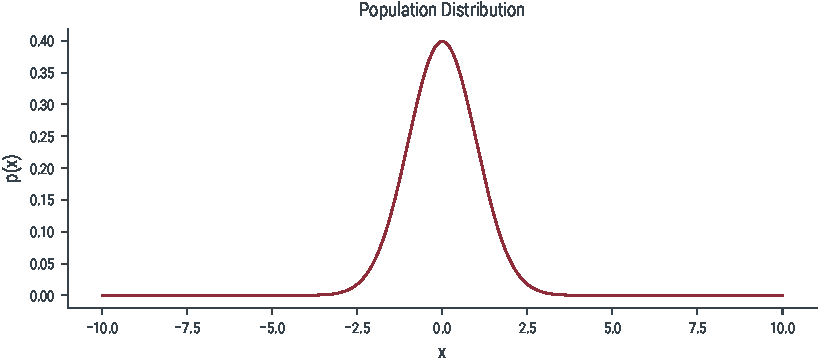
\includegraphics[width=\textwidth]{../figures/mle/population-dist.pdf}
        
    \end{frame}

    \begin{frame}{Population v/s Sample}
        Entire population:
        $$\infty \texttt{ samples from } \mathcal{N}(\mu, \sigma^2)$$
        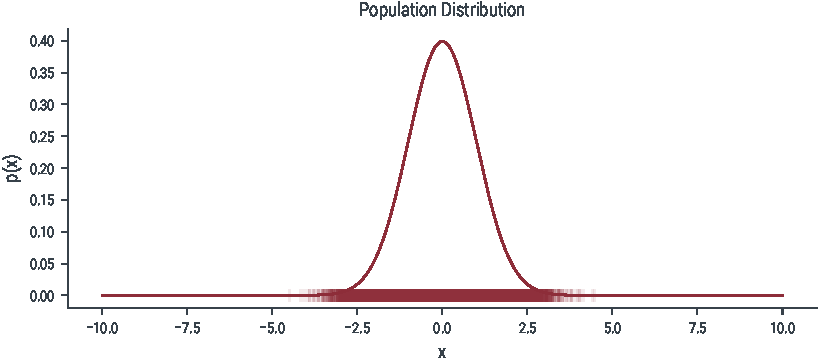
\includegraphics[width=\textwidth]{../figures/mle/population.pdf}
        
    \end{frame}

    \begin{frame}{Population v/s Sample}
        Goal estimate of parameters $\mu$ and $\sigma^2$ from a sample:
        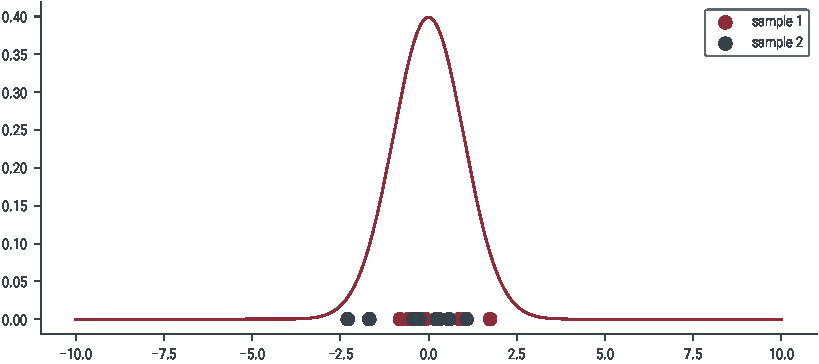
\includegraphics[width=\textwidth]{../figures/mle/sample.pdf}
        
    \end{frame}

    \begin{frame}
        Notebook (mle-biased.ipynb)
    \end{frame}
    


     % Define a loop for each set of figures
\newcommand{\insertfigures}[2]{
    \foreach \i in {0,1,2,3,4,5}{
        \begin{frame}{Sample Size = #1, Sample Number = \i}
            \begin{figure}
                \includegraphics[width=\textwidth]{../figures/mle/biased-mle-normal-#1-\i.pdf}
            \end{figure}
        \end{frame}
    }
    \begin{frame}{Quality of Estimate from Sample Size = #1}
        \begin{figure}
            \includegraphics[width=\textwidth]{../figures/mle/biased-mle-normal-scatter-#2.pdf}
        \end{figure}
    \end{frame}
}

% Call the loop for each set of figures
\insertfigures{3}{3}
\insertfigures{4}{4}
\insertfigures{5}{5}
\insertfigures{10}{10}
\insertfigures{100}{100}


\begin{frame}{Quality of Estimate (of Variance) v/s Sample Size (N)}
    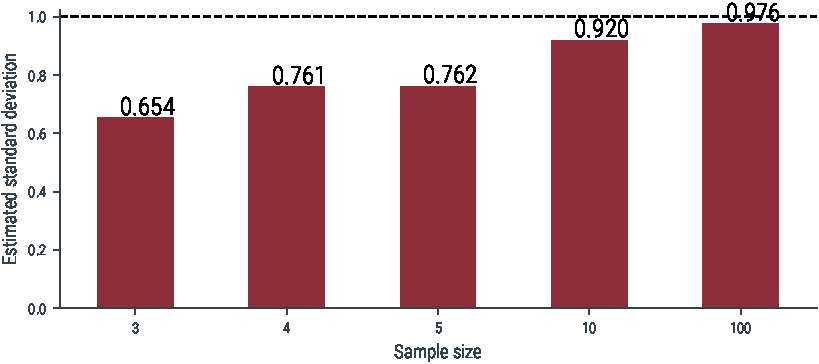
\includegraphics[width=\textwidth]{../figures/biased-mle-variance-quality.pdf}
\end{frame}

\begin{frame}{Quality of Estimate (of Variance) v/s Sample Size (N)}
    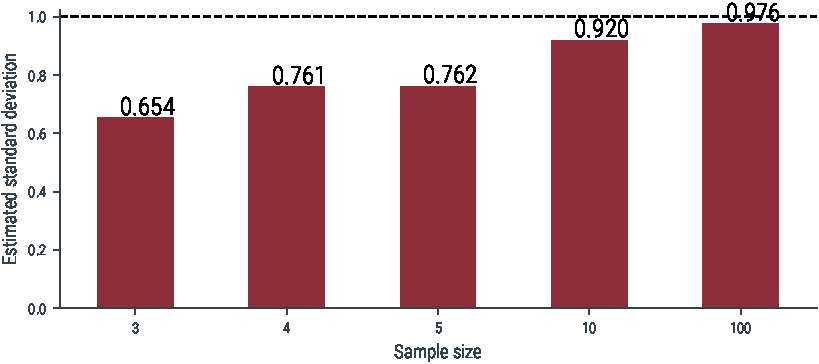
\includegraphics[width=\textwidth]{../figures/biased-mle-variance-quality.pdf}
Can you think of a way to improve the estimate of variance? 
Hint: Think of some function of the number of samples.
\end{frame}

\begin{frame}{Quality of Estimate (of Variance) v/s Sample Size (N)}
    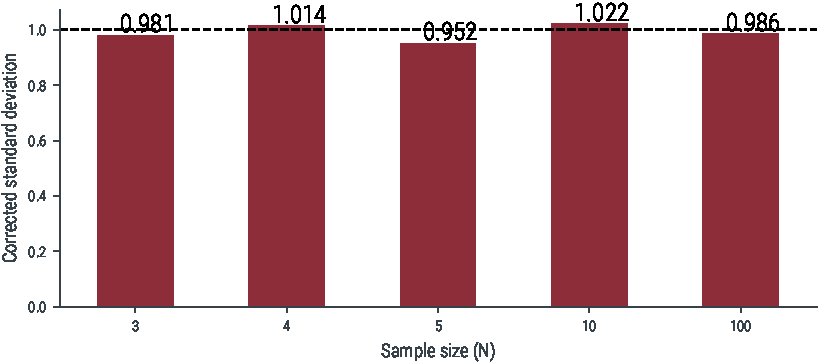
\includegraphics[width=\textwidth]{../figures/corrected-mle-variance-quality.pdf}
Correction multiplactive factor for variance:
\[
    \frac{N}{N-1}
\]
\end{frame}
    

\begin{frame}{Bias of an Estimator}
    \begin{tcolorbox}[colback=metropolisblue!5,colframe=metropolisblue,title=Bias of an Estimator]
        The bias of an estimator $\hat{\theta}$ of a parameter $\theta$ is defined as:
        \[
            \text{Bias}(\hat{\theta}) = \mathbb{E}(\hat{\theta}) - \theta
        \]
        where $\mathbb{E}(\hat{\theta})$ is the expected value of the estimator $\hat{\theta}$.
    \end{tcolorbox}
    \begin{itemize}
        \item An estimator is said to be unbiased if $\text{Bias}(\hat{\theta}) = 0$.
        \item An estimator is said to be biased if $\text{Bias}(\hat{\theta}) \neq 0$.
    \end{itemize}
    
\end{frame}


\begin{frame}{Bias of an Estimator: Relation to Bias-Variance Tradeoff in ML}
    \href{https://nipunbatra.github.io/ml2023/lectures/cross-validation.pdf}{Slides from ML course}
\end{frame}

\begin{frame}{Bias of an Estimator: Relation to SGD}
    \href{https://florian.github.io/estimators/}{Link from ML course}
\end{frame}

    
\begin{frame}{Bias of an Estimator: $\hat{\mu}_{MLE}$}

    \href{https://online.stat.psu.edu/stat415/lesson/1/1.3}{Reference}
        
    % \begin{align*}
    %     \mathbb{E}(\hat{\mu}_{MLE}) &= \mathbb{E}(\Bar{X}) \\
    %     &=\mathbb{E}\left(\frac{1}{n}\sum_{i=1}^nX_i\right) \\
    %     &=\frac{1}{n}\sum_{i=1}^n\mathbb{E}(X_i) \\
    %     &=\frac{1}{n}(n\mu) = \mu
    % \end{align*}
    
    
    % % Add tcolorbox here
    % \begin{tcolorbox}[colback=metropolisblue!5,colframe=metropolisblue,title= Estimator $\hat{\mu}_{MLE}$ is unbiased]
    %     $\mathbb{E}(\hat{\mu}_{MLE}) = \mu$
    % \end{tcolorbox}

    
\end{frame}
\begin{frame}{MLE for Bernoulli Distribution}
    The probability mass function of a bernoulli distribution is given by:
    
    \begin{equation}
    f(x|\theta) = \theta^x(1-\theta)^{(1-x)}
    \end{equation}
    
    Let us assume we have a dataset $D = \{x_1, x_2, \ldots, x_n\}$, where each $x_i$ is an independent sample from the above distribution and $x_i\in\{0, 1\}$.
    We want to estimate the parameter $\theta$ from the data.
    
    Our likelihood function is given by:
    \begin{equation}
    P(D|\theta) = \mathcal{L}(\theta) = \prod_{i=1}^n f(x_i|\theta)
    \end{equation}
    \end{frame}



    \begin{frame}{Graphical model}
        Assume model parameters are $\theta$ and data is $D  $. We can write the joint probability distribution as:

        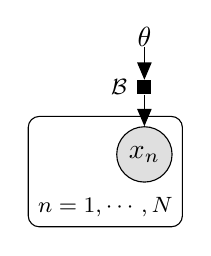
\begin{tikzpicture}
                
                
            \node[obs]                               (xn) {$x_n$};
            \factor[above=of xn] {y-f} {left:${\mathcal{B}}$} {} {} ; %
            \node[const, above=1 of xn] (theta) {$\mathbf{\theta}$};
            \plate{}{(xn)}{$n = 1, \cdots, N$};
            
            
            
            \edge {y-f} {xn} ; %
            \edge {theta} {y-f} ; %
            
            
        \end{tikzpicture}
        
    \end{frame}
    
    \begin{frame}{Log Likelihood Function}
        Log-likelihood function:
        \begin{equation}
            \log \mathcal{L}(\theta) = \sum_{i=1}^n \log f(x_i|\theta)
        \end{equation}
    
        Simplifying the above equation, we get:
        \begin{align*}
            \log \mathcal{L}(\theta) &= \sum_{i=1}^n \log f(x_i|\theta) \\
            &= \sum_{i=1}^n \log \left (\theta^{x_{i}}(1-\theta)^{(1-x_{i})} \right) \\
            &= \sum_{i=1}^n \left( \log \left( \theta^{x_{i}} \right) + \log \left( (1-\theta)^{(1-x_{i})}  \right) \right) \\
            \end{align*}
    \end{frame}
    \begin{frame}
       
        \begin{align*}
            \log \mathcal{L}(\theta) &= \sum_{i=1}^n \left (x_{i}\log \left( \theta \right) + (1-x_{i})\log \left(1-\theta \right) \right)\\
            \end{align*}
            \begin{tcolorbox}[colback=metropolisblue!5,colframe=metropolisblue,title=Log Likelihood Function for Bernoulli Distribution]
                Log-likelihood function for bernoulli distributed data is:
                \[
                    \log \mathcal{L}(\theta) = \sum_{i=1}^n  (x_{i}\log(\theta) + (1-x_{i})\log(1-\theta))
                    \]
            \end{tcolorbox}
    \end{frame}
    
    \begin{frame}
        \frametitle{Maximum Likelihood Estimate for $\theta$}
        
        To find the MLE for $\theta$, we differentiate the log-likelihood function with respect to $\theta$ and set it to zero:
        
        \begin{align*}
            \frac{\partial \log \mathcal{L}(\theta)}{\partial \theta} &= \frac{\partial}{\partial \theta} \left (\sum_{i=1}^n \left (x_{i}\log \left( \theta \right) + (1-x_{i})\log \left(1-\theta \right) \right)\right)\\
            &= \sum_{i=1}^n \left (\frac{\partial}{\partial \theta}(x_{i}\log \left( \theta \right)) + \frac{\partial}{\partial \theta}(1-x_{i})\log \left(1-\theta \right) \right)\\
            &= \sum_{i=1}^n \left (x_{i}\frac{\partial}{\partial \theta}\log \left( \theta \right) + (1-x_{i})\frac{\partial}{\partial \theta}\log \left(1-\theta \right) \right)\\
            &= \sum_{i=1}^n \left (\frac{x_{i}}{\theta} - \frac{(1-x_{i})}{1-\theta} \right)=0\\
        \end{align*}
        
        
        \end{frame}
    
    \begin{frame}
            
        \begin{align*}
            \frac{\partial \log \mathcal{L}(\theta)}{\partial \theta} &=  \sum_{i=1}^n \left (\frac{x_{i}(1-\theta)-\theta(1-x_{i})}{\theta(1-\theta)} \right)=0\\
            &= \sum_{i=1}^n \left (\frac{x_{i}-x_{i}\theta-\theta+\theta x_{i}}{\theta(1-\theta)} \right)\\
            &= \sum_{i=1}^n \left (\frac{x_{i}-\theta}{\theta(1-\theta)} \right)\\
            &= \sum_{i=1}^n \left (x_{i}-\theta \right)=0\\
            &= \sum_{i=1}^n x_{i} - \sum_{i=1}^n\theta=0\\
            &= \sum_{i=1}^n x_{i} - n\theta=0\\
        \end{align*}
        
        
        \end{frame}
    
    \begin{frame}
            
        \begin{align*}
            \theta=\frac{\sum_{i=1}^n x_{i}}{n}\\
        \end{align*}
        \begin{tcolorbox}[colback=metropolisblue!5,colframe=metropolisblue,title=Maximum Likelihood Estimate for $\theta$]
            MLE of $\theta$, denoted as $\hat{\theta}_{\text{MLE}}$, is given by:
            \begin{equation*}
                \hat{\theta}_{\text{MLE}} = \frac{\sum_{i=1}^n x_{i}}{n}
            \end{equation*}
        \end{tcolorbox}
        
        \end{frame}
    
    \begin{frame}
    For example if we have a Bernoulli Distribution with $\theta=0.2,$ the likelihood, $P(D|\theta)$ is given below:
    \begin{figure}
                    \centerline{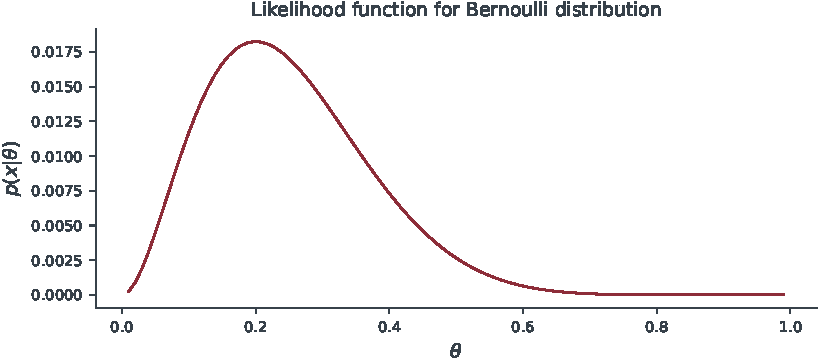
\includegraphics[scale = 0.75]{../figures/mle/bernoulli_likelihood.pdf}}
    \end{figure}
        
    \end{frame}

    \section{MLE for Multivariate Normal Distribution}
\begin{frame}{MLE for Multivariate Normal Distribution}
The probability density function of a multivariate normal distribution is given by:

\begin{equation}
f(x|\mu, \Sigma) = (2\pi)^{-\frac{k}{2}}\det(\Sigma)^{-\frac{1}{2}}exp^{-\frac{1}{2}(x-\mu)^{T}\Sigma^{-1}(x-\mu)}
\end{equation}

Let us assume we have a dataset $D = \{x_1, x_2, \ldots, x_n\}$, where each $x_i$ is an independent sample from the above distribution.
We want to estimate the parameters $\theta = {\mu, \sigma}$ from the data.

Our likelihood function is given by:
\begin{equation}
P(D|\theta) = \mathcal{L}(\mu, \Sigma) = \prod_{i=1}^n f(x_i|\mu, \Sigma)
\end{equation}

\end{frame}

\begin{frame}
    For example: A bivariate Normal distribution can be visualized as given below:
    \begin{figure}
                \centerline{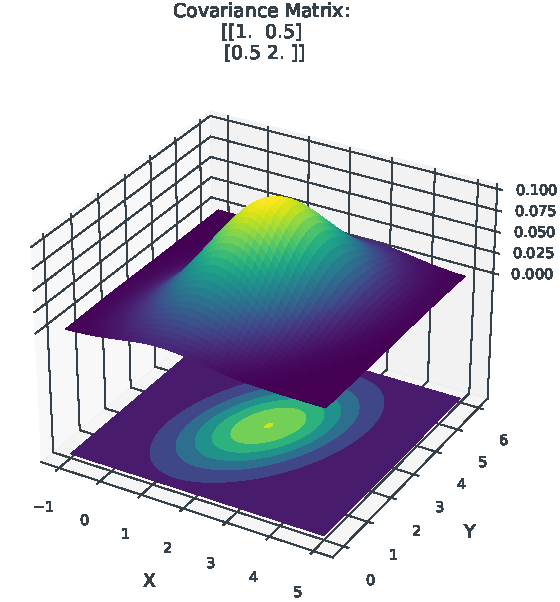
\includegraphics[scale = 0.75]{../figures/mle/bivariate_normal.pdf}}
\end{figure}
    
\end{frame}

\begin{frame}{Log Likelihood Function}
    Log-likelihood function:
    \begin{equation}
        \log \mathcal{L}(\mu, \Sigma) = \sum_{i=1}^n \log f(x_i|\mu, \Sigma)
    \end{equation}

    Simplifying the above equation, we get:
    \begin{align*}
        \log \mathcal{L}(\mu, \Sigma) &= \sum_{i=1}^n \log f(x_i|\mu, \Sigma) \\
        &= \sum_{i=1}^n \log \left((2\pi)^{-\frac{k}{2}}\det(\Sigma)^{-\frac{1}{2}}exp^{-\frac{1}{2}(x_i-\mu)^{T}\Sigma^{-1}(x_i-\mu)} \right) \\
        &= \sum_{i=1}^n \log ((2\pi)^{-\frac{k}{2}}) + \sum_{i=1}^n \log (\det(\Sigma)^{-\frac{1}{2}}) + \\ & \ \ \ \sum_{i=1}^n \log(exp^{-\frac{1}{2}(x_i-\mu)^{T}\Sigma^{-1}(x_i-\mu)} )) 
        \end{align*}
\end{frame}

\begin{frame}
    Continuing, we get:
    \begin{align*}
        = -\frac{kn}{2}\log(2\pi) -\frac{n}{2}\log(\Sigma) -\frac{1}{2}\sum_{i=1}^n (x_i-\mu)^T\Sigma^{-1}(x_i-\mu)  
        \end{align*}

    \begin{tcolorbox}[colback=metropolisblue!5,colframe=metropolisblue,title=Log Likelihood Function for Multivariate Normal Distribution]
            Log-likelihood function for multivariate normally distributed data is:
            \[
                -\frac{kn}{2}\log(2\pi) -\frac{n}{2}\log(\Sigma) -\frac{1}{2}\sum_{i=1}^n (x_i-\mu)^T\Sigma^{-1}(x_i-\mu)
                \]
        \end{tcolorbox}
\end{frame}

\begin{frame}
    \frametitle{Maximum Likelihood Estimate for $\mu$}
    
    To find the MLE for $\mu$, we differentiate the log-likelihood function with respect to $\mu$ and set it to zero:
    
    \begin{align*}
      &=\frac{\partial}{\partial \mu} \left(-\frac{kn}{2}\log(2\pi) -\frac{n}{2}\log(\Sigma) -\frac{1}{2}\sum_{i=1}^n (x_i-\mu)^T\Sigma^{-1}(x_i-\mu)\right) \\
      &= \frac{\partial}{\partial \mu} \left(-\frac{1}{2} \sum_{i=1}^n (x_i-\mu)^T\Sigma^{-1}(x_i-\mu)\right) \\
      &= -\frac{1}{2}\sum_{i=1}^n \left(\Sigma^{-1}(x_i-\mu) + (x_i-\mu)^T\Sigma^{-1} \right) = 0\\
      &= -\frac{1}{2} \sum_{i=1}^n 2\Sigma^{-1}(x_i-\mu) = 0 
    \end{align*} \centerline{as $(x_i-\mu)^{T}\Sigma^{-1} = \Sigma^{-1}(x_i-\mu)$}
    
\end{frame}

\begin{frame}
    
    \begin{align*}
      &=\Sigma^{-1}\sum_{i=1}^n(x_i-\mu) = 0 \\
      &=\sum_{i=1}^n(x_i) - n\mu = 0 \\
      &\mu = \frac{\sum_{i=1}^n x_i}{n}      
    \end{align*} 

    \begin{tcolorbox}[colback=metropolisblue!5,colframe=metropolisblue,title=Maximum Likelihood Estimate for $\mu$]
        MLE of $\mu$, denoted as $\hat{\mu}_{\text{MLE}}$, is given by:
        \begin{equation*}
            \hat{\mu}_{\text{MLE}} = \frac{1}{n}\sum_{i=1}^n x_i
        \end{equation*}
    \end{tcolorbox}
    
\end{frame}

\begin{frame}{MLE for $\Sigma$ for multivariate normally distributed data}
    Recall that the log-likelihood function is given by:
    \begin{equation}
        \log \mathcal{L}(\mu, \Sigma) = \sum_{i=1}^n \log f(x_i|\mu, \Sigma)
    \end{equation}

    Let us find the maximum likelihood estimate of $\Sigma$ now. We can do this by taking the derivative of the log-likelihood function with respect to $\Sigma$ and equating it to zero.   

    \begin{equation}
        \frac{\partial \log \mathcal{L}(\mu, \Sigma)}{\partial \Sigma} = \sum_{i=1}^n \frac{\partial \log f(x_i|\mu, \Sigma)}{\partial \Sigma} = 0
    \end{equation}
    
\end{frame}
\begin{frame}
    After differentiating and simplifying, we get:
    \begin{align*}
      \Sigma = \frac{1}{n}\sum_{i=1}^n(x_i-\mu)(x_i-\mu)^T  
    \end{align*} 

    \begin{tcolorbox}[colback=metropolisblue!5,colframe=metropolisblue,title=Maximum Likelihood Estimate for $\Sigma$]
        MLE of $\Sigma$, denoted as $\hat{\Sigma}_{\text{MLE}}$, is given by:
        \begin{equation*}
            \hat{\Sigma}_{\text{MLE}} = \frac{1}{n}\sum_{i=1}^n (x_i-\mu)(x_i-\mu)^T
        \end{equation*}
    \end{tcolorbox}
\end{frame}

    
    
    

% \begin{frame}
%     \frametitle{References}

%     \begin{enumerate}
%         \item \href{https://stats.stackexchange.com/questions/239500/what-is-the-difference-between-random-variable-and-random-sample#:~:text=A%20random%20sample%20is%20to,experiment%20to%20a%20real%20number}{Random Variable v/s Random Sample}
%         \item \href{https://online.stat.psu.edu/stat415/lesson/1/1.3}{Biased and Unbiased Estimators}
%     \end{enumerate}
% \end{frame}

% \begin{frame}{Bias of an Estimator: $\hat{\mu}_{MLE}$}
%     \pause 
%     Question: What is the expectation of $\hat{\mu}_{MLE}$ calculated over? What is the source of randomness?
    
%     Let us assume that the true underlying distribution is $\mathcal{N}(\mu, \sigma^2)$.

%     Let $\mathcal{D}^1 = \{x^1_1, x^1_2, \ldots, x^1_n\}$ be a dataset obtained from this distribution. 

%     The MLE of $\mu$ based on $\mathcal{D}^1$ is given by:
%     \begin{align*}
%         \hat{\mu}_{MLE}^1 = \frac{1}{n} \sum_{i=1}^n x^1_i
%     \end{align*}

%     If we obtained another dataset $\mathcal{D}^2 = \{x^2_1,  x^2_2, \ldots, x^2_n\}$ from the same distribution, the MLE of $\mu$ based on $\mathcal{D}^2$ would be:
%     \begin{align*}
%         \hat{\mu}_{MLE}^2 = \frac{1}{n} \sum_{i=1}^n x^2_i
%     \end{align*}
% \end{frame}

% \begin{frame}{Bias of an Estimator: $\hat{\mu}_{MLE}$}
%     If we repeat this process and obtain datasets $\mathcal{D}^1, \mathcal{D}^2, \ldots, \mathcal{D}^k$, we would have $k$ different estimates of $\mu$.

%     Taking the expectation of these $k$ estimates gives us the expected value of $\hat{\mu}_{MLE}$:
%     \begin{align*}
%         \mathbb{E}(\hat{\mu}_{MLE}) = \frac{1}{k} \sum_{i=1}^k \hat{\mu}_{MLE}^i
%     \end{align*}

%     Simplifying further, we have:
%     \begin{align*}
%         \mathbb{E}(\hat{\mu}_{MLE}) = \frac{1}{kn} \sum_{i=1}^k \sum_{j=1}^n x^i_j
%     \end{align*}
    
%     This expectation is calculated over multiple datasets $\mathcal{D}^1, \mathcal{D}^2, \ldots, \mathcal{D}^k$, where each dataset represents a different realization of the random variables from the underlying distribution.
    
   
% \end{frame}

% \begin{frame}{Bias of an Estimator: $\hat{\mu}_{MLE}$}
%     To show that the estimator $\hat{\mu}_{MLE}$ is unbiased, we need to demonstrate that $\mathbb{E}(\hat{\mu}_{MLE}) = \mu$.
    
%     Recall that each $x^i_j$ is a random variable following $\mathcal{N}(\mu, \sigma^2)$. Therefore, the sum $\sum_{i=1}^k x^i_j$ follows $\mathcal{N}(k\mu, k\sigma^2)$.
    
%     Thus, we can write:
%     \begin{align*}
%         \mathbb{E}(\hat{\mu}_{MLE}) &= \frac{1}{kn} \sum_{i=1}^k \sum_{j=1}^n x^i_j = \frac{1}{kn} \sum_{j=1}^n \left(\sum_{i=1}^k x^i_j\right) \\
%         &= \frac{1}{kn} \sum_{j=1}^n (k\mu) = \frac{1}{kn} (kn\mu) =\mu
%     \end{align*}
    
%     % Add tcolorbox here
%     \begin{tcolorbox}[colback=metropolisblue!5,colframe=metropolisblue,title= Estimator $\hat{\mu}_{MLE}$ is unbiased]
%         $\mathbb{E}(\hat{\mu}_{MLE}) = \mu$
%     \end{tcolorbox}

    
% \end{frame}

% \begin{frame}
%     \frametitle{Bias of $\sigma^2_{MLE}$}
    
%     The MLE of $\sigma^2$ is given by
    
%     $\hat{\sigma}^2_{MLE} = \frac{1}{n} \sum_{i=1}^n (x_i-\mu)^2$ where $\mu$ is the MLE of the mean.
    
%     \begin{align*}
%         \mathbb{E}(\hat{\sigma}^2_{MLE}) &= \mathbb{E}\left[\frac{1}{n} \sum_{i=1}^n (x_i-\mu)^2\right] = \frac{1}{n} \sum_{i=1}^n \mathbb{E}[(x_i-\mu)^2] \\
%         &= \frac{1}{n} \sum_{i=1}^n \mathbb{E}[x_i^2] - 2\mu \mathbb{E}[x_i] + \mu^2 = \frac{1}{n} \sum_{i=1}^n \sigma^2 + \mu^2 - 2\mu \mu \\
%         &= \frac{n-1}{n} \sigma^2 + \mu^2 - \mu^2 = \frac{n-1}{n} \sigma^2
%         \end{align*}

%         \begin{tcolorbox}[colback=metropolisblue!5,colframe=metropolisblue,title= Estimator $\hat{\sigma}^2_{MLE}$ is biased]
%             $\mathbb{E}(\hat{\sigma}^2_{MLE}) = \frac{n-1}{n} \sigma^2$
%         \end{tcolorbox}

%     \end{frame}
    


    

\end{document}